\chapter{Countdown}
Countdown is a well-known functional programming puzzle (with a spin-off TV show
in the UK), first popularised as a puzzle in which to demonstrate functional
algorithms in \cite{huttonCountdownProblem2002}.
The idea is simple: given a list of numbers, contestants must construct an
arithmetic expression (using a small set of functions) using some or all of the
numbers, to reach some target.

Take the following problem as an example:
\begin{gather*}
  \boxed{1} \boxed{3} \boxed{7} \boxed{10} \boxed{25} \boxed{50} \\
  \boxed{765} \tag{Target}
\end{gather*}
It has the following answer:
\begin{equation}
  3 \times ((7 \times (50 - 10)) - 25)
\end{equation}
Importantly, we do not have to use every number given to get to the target.
For our problem, we will use the operators \(\times\), \(+\), and \(-\).

In this section we will develop a program/proof which can decide countdown
problems totally.
In other words, given a list of numbers and a target, our program will prove
whether a solution exists, and if so, it will provide just that solution.
\section{Classifying The Problem}
So what is a ``solution'' to the countdown problem?
Given some list of numbers, what type classifies the candidates for testing from
those numbers?
What is the type of the following transformation?
\begin{alignat*}{6}
  &1 \; \; \;         &&3         &&7    &&10    &&25  &&50 \\
  &&&3 \times (&&7 \times (&&50 - &&10) - &&25)
\end{alignat*}
Firstly, we can notice that not every number was used in our solution.
So the transformation must information about what to keep and what to discard on
an item-by-item basis: a subsequence, in other words.
% \begin{align*}
%   &1 \; \; \;         &&3         &&7    &&10    &&25  &&50 \\
%   &         &&3         &&7    &&10    &&25  &&50 \\
%   &         &&3         &&7    &&50    &&10  &&25 \\
%   &         &&3   \times      &&7 \times    &&50 -    &&10 -  &&25 \\
%   &&&3 \times ((&&7 \times (&&50 - &&10)) - &&25)
% \end{align*}

  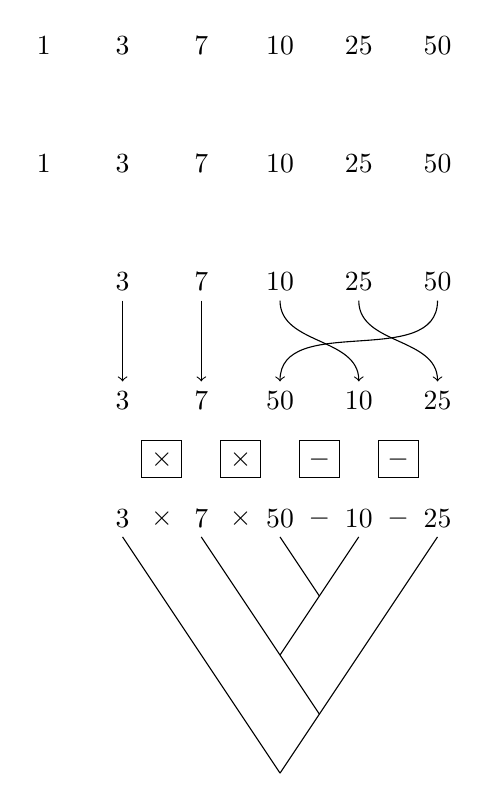
\begin{tikzpicture}

    \node at (-1,  3) {1}  ;
    \node at (0 ,  3) {3}  ;
    \node at (1 ,  3) {7}  ;
    \node at (2 ,  3) {10} ;
    \node at (3 ,  3) {25} ;
    \node at (4 ,  3) {50} ;

    \node at (-1,  1.5) {\xcancel{1}}  ;
    \node at (0 ,  1.5) {3}  ;
    \node at (1 ,  1.5) {7}  ;
    \node at (2 ,  1.5) {10} ;
    \node at (3 ,  1.5) {25} ;
    \node at (4 ,  1.5) {50} ;

    \node(t3)   at (0 ,  0) {3}  ;
    \node(t7)   at (1 ,  0) {7}  ;
    \node(t10)  at (2 ,  0) {10} ;
    \node(t25)  at (3 ,  0) {25} ;
    \node(t50)  at (4 ,  0) {50} ;
    \node(b3)   at (0 , -1.5) {3}  ;
    \node(b7)   at (1 , -1.5) {7}  ;
    \node(b50)  at (2 , -1.5) {50} ;
    \node(b10)  at (3 , -1.5) {10} ;
    \node(b25)  at (4 , -1.5) {25} ;

    \draw [->, rounded corners] (t3.south) --  (b3.north) ;
    \draw [->, rounded corners] (t7.south) --  (b7.north) ;
    \draw [->, rounded corners] (t10.south) to[out=-90, in=90] (b10.north) ;
    \draw [->, rounded corners] (t25.south) to[out=-90, in=90] (b25.north) ;
    \draw [->, rounded corners] (t50.south) to[out=-90, in=90] (b50.north) ;


    \node[draw] at (0.5 , -2.25) {$\times$} ;
    \node[draw] at (1.5 , -2.25) {$\times$} ;
    \node[draw] at (2.5 , -2.25) {$-$} ;
    \node[draw] at (3.5 , -2.25) {$-$} ;

    \node at (0.5 , -3) {$\times$} ;
    \node at (1.5 , -3) {$\times$} ;
    \node at (2.5 , -3) {$-$} ;
    \node at (3.5 , -3) {$-$} ;

    \node(e3) at (0   , -3) {3}  ;
    \node(e7) at (1   , -3) {7}  ;
    \node(e50) at (2   , -3) {50} ;
    \node(e10) at (3   , -3) {10} ;
    \node(e25) at (4   , -3) {25} ;

    \draw[-] (e50.south) -- ++(0.5,-0.75 ) ;
    \draw[-] (e10.south) -- ++(-1 ,-1.5  ) ;
    \draw[-] (e7.south)  -- ++(1.5,-2.25) ;
    \draw[-] (e3.south)  -- ++(2  , -3 ) ;
    \draw[-] (e25.south) -- ++(-2 , -3 ) ;
  \end{tikzpicture}


\section{Enumerating Combinations and Permutations}
\section{Enumerating Binary Trees}
\section{Filtering Out Invalid Expressions with the Subobject Classifier}
\section{Filtering Out Duplicates with Quotients}


%%% Local Variables:
%%% mode: latex
%%% TeX-master: "../paper"
%%% End: